%instiki:category: QuantumFieldTheory
\chapter{Two body decays}
\label{cha:two-body-decays} %noinstiki
%instiki:
%instiki:***
%instiki:
%instiki:[[Beyond|Contents]]
%instiki:
%instiki:***
%instiki:
%instiki:* [Particle decays](#particle-decays)
%instiki:
%instiki:* [Width decay](#width-decay)
%instiki:
%instiki:* [Feynman Rules and trace theorems](#feynman-rules-trace)
%instiki:

In this chapter we use directly the Feynman rules for Fermions to carry out the calculation of the decay of the standard model Higgs into a pair of fermions. In chapter \ref{chap:fr} we will obtain the corresponding Feynman rules from the $S$--matrix expansion.




\section{Particle decays}
\label{sec:particle-decays}

Particle decay \cite{PD}  is the spontaneous process of one elementary particle transforming into other elementary particles. During this process, an elementary particle becomes a different particle with less mass and an intermediate particle such as $W$ boson in muon decay. 

For a particle of a mass $M$,  the differential decay width according Eq.~\eqref{eq:51}, is
\begin{equation}
  \label{eq:76}
 d\Gamma_n = \frac{(2\pi)^4}{2M}\left|\mathcal{M}\right|^2 d \Phi^{(n)} (P; p_1, p_2,\dots, p_n) \,
\end{equation}
The phase space can be determined from Eq.~\eqref{eq:50}
\begin{equation}
  d \Phi^{(n)} (P; p_1, p_2,\dots, p_n) = \delta^4 (P - \sum_{i=1}^n p_i) \left( \prod_{i=1}^n \frac{d^3 p_i}{(2\pi)^3 2 E_i} \right)\,.
\end{equation}
We will keep the $d\Gamma$ notation until all the integrals get evaluated. 

The two-body decays in eq.~\eqref{eq:152} is 
\begin{align}
\label{eq:154}
\frac{d\Gamma}{d\Omega}=
&\frac{1}{64 \pi^2M^3}\left|\mathcal{M}_{fi}\right|^2\lambda^{1/2}(M^2,m_2^2,m_1^2)\end{align}



\section{Width decay}
\label{sec:width-decay}
%Poner las reglas de Feynman Aqui

Reglas de Feynman: Time direction from left to right.
\begin{itemize}
\item Initial particle: ${u}(p)$ 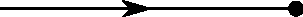
\includegraphics{frip}
\item Initial antiparticle: $\bar{v}(p)$ 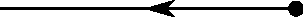
\includegraphics{fria}
\item Final particle: $\bar{u}(p)$ 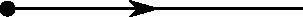
\includegraphics{frfp}
\item Final antiparticle: ${v}(p)$ 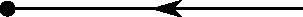
\includegraphics{frfa}

\end{itemize}

We consider now a general Yukawa interaction term
\begin{align}
  \mathcal{L}_{\text{int}}=hH\overline{f}_1 f_2
\end{align}
For the $H\to \overline{f}_1f_2$ decay.
The interaction between the Higgs boson with fermions\footnote{In this case we consider only electrons, by the formula is easy generalizable to other fermions} is given by the Yukawa interaction term \cite{lsm}
\begin{align}
\label{eq:155}
\mathcal{L}_{\text{Higgs}}&=-G_{f}\frac{(v+H)}{\sqrt{2}}(\overline{f}_{R}f_{L}+\overline{f}_{L}f_{R})\nonumber\\
&=-\frac{G_{f}v}{\sqrt{2}}\overline{f}f-\frac{G_{f}H}{\sqrt{2}}\overline{f}f\nonumber\\
&=-m_f\overline{f}f-m_f\left(G_{F}\sqrt{2}\right)^{1/2}\overline{f}f
\end{align}
Such as the electro has acquired a mass $m_{e}=G_{f}\nu/\sqrt{2}$. On the other hand the coupling to be assigned to the process vertex is 
$G_{f}\sqrt{2}$ or $m_{f}/v=$. 

The decay process $H\to f\overline{f}$, is displayed in Fig. 
\ref{fig:a} %noinstiki

\begin{figure}[h!] %noinstiki
\begin{center} %noinstiki
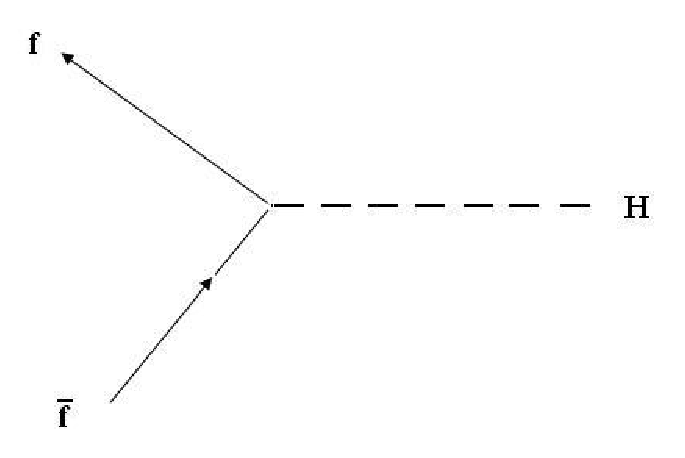
\includegraphics[scale=0.5]{decay}%noinstiki
\caption{Diagrama de proceso $H\to f\overline{f}$} %noinstiki
\label{fig:a} %noinstiki
\end{center} %noinstiki
\end{figure} %noinstiki

The Feynman rules, to be explained in Chapter~\ref{chap:fr} are indicated in Fig. 
\ref{fig:b}. %noinstiki

\begin{figure}[h] %noinstiki
\begin{center} %noinstiki
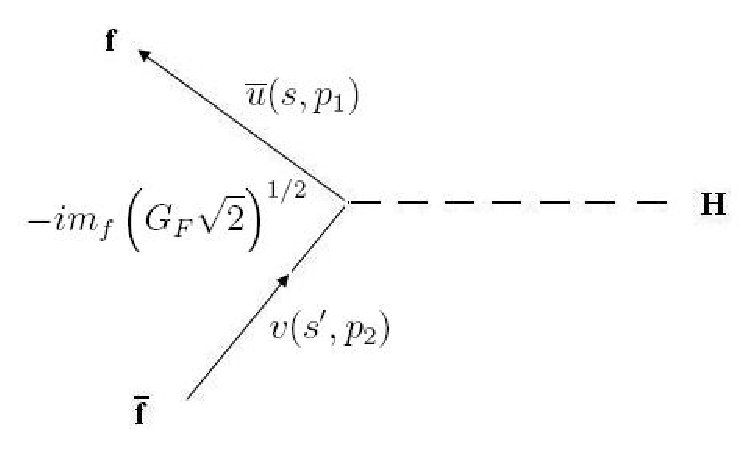
\includegraphics[scale=0.65]{feyn}%noinstiki
\caption{Reglas de Feynman del proceso $H\to f\overline{f}$}%noinstiki
\label{fig:b} %noinstiki
\end{center} %noinstiki
\end{figure} %noinstiki

In this way the scattering amplitude is 
\begin{equation}
i\mathcal{M}=-im_{f}\left(G_{F}\sqrt{2}\right)^{1/2}\overline{u}(s_1,
p_{1})v(s_2, p_{2}). 
\end{equation}
where $p_{1}$, $s$,  $p_{2}$ y $s_2$ are the momentum and spines of fermion and anti--fermion respectively.

For the general case
\begin{align}
i\mathcal{M}=-i h\overline{u}(s_1,p_{1})v(s_2, p_{2}). 
\end{align}
$h=m_{f}\left(G_{F}\sqrt{2}\right)^{1/2}$ in the standard models
Now, having into account that ${\gamma^{0}}^{\dag}=\gamma^{0}$
\begin{align*}
&(\overline{u}(s_1,p_{1})v(s_2, p_{2}))^{\dag}\\
&=v^{\dag}(s_2, p_{2})(\overline{u}(s_1,p_{1}))^{\dag}\\
&=v^{\dag}(s_2, p_{2})({u^{\dag}}(s_1,p_{1}){\gamma^{0}})^{\dag}\\
&=v^{\dag}(s_2, p_{2})({\gamma^{0}}^{\dag}u(s_1,p_{1}))\\
&=v^{\dag}(s_2, p_{2})(\gamma^{0}u(s_1,p_{1}))\\
&=\overline{v}(s_2,p_{2})u(s_1,p_{1}). 
\end{align*}
Squaring  $\mathcal{M}$,  and summing over possible polarization states of final particles, we have

\begin{equation}
\sum_{s_1,s_2}|\mathcal{M}|^{2}=h^2\sum_{s_1,s_2}(\overline{u}(s_1,p_{1})v(s_2,
p_{2}))(\overline{v}(s_2,p_{2})u(s_1,p_{1})). \label{eq:80}
\end{equation}
The several sums in Ec.~(\ref{eq:80}) can be calculated by expressing the products  $\overline{u}v$ y $\overline{v}u$ en in terms of their components, as follow
\begin{align}
\label{eq:81}
&\sum_{s_1,s_2}(\overline{u}(s_1,p_{1})v(s_2, p_{2}))(\overline{v}(s_2,p_{2})u(s_1,p_{1}))\nonumber\\
&=\sum_{s_1,s_2}(\overline{u}_{\alpha}(s_1,p_{1})v_{\alpha}(s_2, p_{2}))(\overline{v}_{\beta}(s_2,p_{2})u_{\beta}(s_1,p_{1}))\nonumber\\
&=\sum_{s_1,s_2}(u_{\beta}(s_1,p_{1})\overline{u}_{\alpha}(s_1,p_{1}))(v_{\alpha}(s_2, p_{2})\overline{v}_{\beta}(s_2,p_{2}))\nonumber\\
&=\sum_{s}u_{\beta}(s_1,p_{1})\overline{u}_{\alpha}(s_1,p_{1})\sum_{s_2}v_{\alpha}(s_2, p_{2})\overline{v}_{\beta}(s_2,p_{2})\nonumber\\
&=(\cancel{p}_{1}+m_{f})_{\beta\alpha}(\cancel{p}_{2}-m_{f})_{\alpha\beta}\nonumber\\
&=\operatorname{Tr}[(\cancel{p}_{1}+m_{f})(\cancel{p}_{2}-m_{f})]. 
\end{align}
Taking into account that  $\operatorname{Tr}[\gamma_{\nu}]=0$, and from the commutation relations for $\gamma_\mu$ matrices
\begin{align*}
\operatorname{Tr}[\gamma_{\mu}\gamma_{\nu}]&=tr[-\gamma_{\nu}\gamma_{\mu}+2g^{\mu\nu}]\\
&=\operatorname{Tr}[-\gamma_{\nu}\gamma_{\mu}]+2g^{\mu\nu}\operatorname{Tr}[\mathbf{1}]\\
&=\operatorname{Tr}[-\gamma_{\mu}\gamma_{\nu}]+2g^{\mu\nu}4 \qquad (\operatorname{Tr}[AB]=\operatorname{Tr}[BA])\\
\operatorname{Tr}[\gamma_{\mu}\gamma_{\nu}]&=4g^{\mu\nu}.
\end{align*}

In this way
\begin{align*}
&\operatorname{Tr}[(\cancel{p}_{1}+m_{1})(\cancel{p}_{2}-m_{2})]\\
&=\operatorname{Tr}[(\gamma_{\mu}p^{\mu}_{1}+m_{1})(\gamma_{\nu}p^{\nu}_{2}-m_{1})]\\
&=\operatorname{Tr}[\gamma_{\mu}\gamma_{\nu}p^{\mu}_{1}p^{\nu}_{2}-m_{2}\gamma_{\mu}p^{\mu}_{1}+m_{1}\gamma_{\nu}p^{\nu}_{2}-m_{1}m_2]\\
&=p^{\mu}_{1}p^{\nu}_{2}tr[\gamma_{\mu}\gamma_{\nu}]-4m_1 m_2\\
&=4g_{\mu\nu}p^{\mu}_{1}p^{\nu}_{2}-4m_1m_2\\
&=4(p_{1}\cdot p_{2}-m_1m_2). 
\end{align*}
where  $m_1$, $m_2$ are the final masses, and
\begin{equation*}
\sum_{s_1,s_2}|\mathcal{M}|^{2}=4h^2(p_{1}\cdot p_{2}-m_{1}m_2).
\end{equation*}
From eq.~\eqref{eq:153}
\begin{align}
  M=&E_1+E_2\nonumber\\
|\mathbf{p}_1|&=|\mathbf{p}_2|
\end{align}
Therefore
\begin{align}
  E_1E_2=\frac{M^2-E_1^2-E_2^2}{2}
\end{align}
\begin{align*}
p_{1}\cdot p_{2}-m^{2}_{f}&=E_{1}E_{2}-\mathbf{p}_{1}\cdot\mathbf{p}_{2}-m_1 m_2\\
&=E_{1}E_{2}+\mathbf{p}_{1}^2-m_1 m_2\\
&=\frac{M^2-E_1^2-E_2^2}{2}+\mathbf{p}_{1}^2-m_1 m_2\nonumber\\
&=\frac12\left(M^2-m_1^2-\mathbf{p}_1^2-m_2^2-\mathbf{p}_1^2\right)+\mathbf{p}_{1}^2-m_1 m_2\\
&=\frac12\left(M^2-m_1^2-m_2^2-2m_1m_2\right)\\
&=\frac12\left[M^2-(m_1-m_2)^2\right]
\end{align*}
%\left(\right)
Therefore, the scattering  amplitude is
\begin{equation}
\sum_{s_1,s_2}|\mathcal{M}|^{2}=2h^2\left[M^2-(m_1+m_2)^2\right]
\label{eq:82}
\end{equation}
Replacing back in eq.~\eqref{eq:155}
\begin{align}
\frac{d\Gamma}{d\Omega}=
&\frac{h^2}{32 \pi^2M^3}\lambda^{1/2}(M^2,m_2^2,m_1^2)\left[M^2-(m_1+m_2)^2\right]
\end{align}
After the integration in $d\Omega_{\text{CM}}=4\pi$ we have
\begin{align}
\Gamma=&\frac{h^2}{8 \pi M^3}\lambda^{1/2}(M^2,m_2^2,m_1^2)\left[M^2-(m_1+m_2)^2\right]
\end{align}
For $m_1=m_2=m_f$
\begin{align}
  \lambda^{1/2}(M^2,m_2^2,m_1^2)=&M^2\left(1-\frac{4m_f^2}{M^2}\right)^{1/2}\nonumber\\
\left[M^2-(m_1+m_2)^2\right]=&M^2\left(1-\frac{4m_f^2}{M^2}\right)
\end{align}
and therefore
\begin{align}
\Gamma=&\frac{h^2}{8 \pi}M\left(1-\frac{4m_f^2}{M^2}\right)^{3/2}
\end{align}
In the case of the standard model Higgs with mass $M_H$ decaying to fermion pai, according to the Lagrangian in eq.~\eqref{eq:155}

\begin{equation}
\Gamma(H\to f\overline{f})=\frac{M_{H}m_{f}^{2}G_{F}}{4\pi\sqrt{2}}
\left(1-4\frac{m^2_{f}}{M^2_{H}}\right)^{3/2}, 
\end{equation}

In the limit $m_{f}\ll M_{H}$ this expression reduces to 
\begin{equation}
\Gamma(H\to
f\overline{f})=\frac{M_{H}m_{f}^{2}G_{F}}{4\pi\sqrt{2}}. 
\end{equation}


\section{$e^+ e^- \to \mu^+\mu^-$}

\begin{align}
  \mathcal{L}=\frac{e^2}{s}
  \left[\bar v(k_2)\gamma^\lambda u(k_1)  \right]
  \left[\bar v(k_2)\gamma^\lambda u(k_1)  \right]
\end{align}

%%% Local Variables: 
%%% mode: latex
%%% TeX-master: "beyond"
%%% End: 
